\documentclass[12pt,a4paper]{article}
\usepackage[utf8]{inputenc}
\usepackage[T1]{fontenc}
\usepackage[english]{babel}

\usepackage{geometry}
\geometry{margin=1in}

\usepackage{amsmath}
\usepackage{amssymb}
\usepackage{mathtools}

\usepackage{graphicx}
\usepackage{subcaption}
\usepackage{booktabs}
\usepackage{adjustbox}
\usepackage{float}
\usepackage[style=authoryear]{biblatex}

\usepackage[hidelinks]{hyperref}

\usepackage{setspace}
\onehalfspacing

\addbibresource{reference.bib}

\begin{document}

% ============================================================
\section{Cross Section Risk Sharing}
% ============================================================
Recall that we are focussing our replication exercise on two main outputs. The first output plots (a scaled inverse of) cross-sectional risk-sharing estimates
against the (natural logarithm of) foreign assets over GDP (Figures 1 and 2 in \textcite{main}). It can be regarded as a graphical tool to analyze the co-movement
over time of year-by-year risk-sharing against a measure of financial openness which is likely inversely related to the Home Bias\footnote{The paper does not explain why 
it does not use the Home Bias measure previously described for its plots. We regard it to be a safety measure as the definition of the Equity Home Bias requires 
some more discretionary choice than simply using Foreign Assets over GDP and follow their approach exactly.}.\\
\indent For the cross-sectional risk-sharing regressions, we apply the methodology in \textcite[p.593]{main} which coincides with the standard approach in the literature. 
Specifically, we run regressions of the form:
\begin{equation}
    \Delta \log \mathrm{GNI}_{it}-\Delta \log \mathrm{GNI}_t = \text{constant} + \beta_{K,t}(\Delta \log \mathrm{GDP}_{it}-\Delta\log \mathrm{GDP}_t) + \varepsilon_{it},
\end{equation}
where $\mathrm{GNI}_{it}$ and $\mathrm{GDP}_{it}$ respectively measure per capita Gross Domestic Income and Gross Domestic Product of country i at year t.
$\mathrm{GNI}_t$ and $\mathrm{GDP}_t$ denote the respective aggreagtes over the sample group at year t. Similarly, we run:
\begin{equation}
    \Delta \log \mathrm{C}_{it}-\Delta \log \mathrm{C}_t = \text{constant} + \beta_{C,t}(\Delta \log \mathrm{GDP}_{it}-\Delta\log \mathrm{GDP}_t) + \varepsilon_{it},
\end{equation}
where $\mathrm{C}$ denotes (aggregate or country-level) per capita consumption.\\
\indent Just as in \textcite[p.21]{notes}, we may interpret $\beta_{j,t}=0, j\in\{C,K\}$ as the perfect risk-sharing benchmark. In this case,
idiosyncratic consumption growth perfectly tracks aggregate consumption growth and a country is fully insured against idiosyncratic output shocks.\\
\indent For completeness, we may conclude with the following remark. While consumers ultimately derive utility from consumption, equation (1) may be useful
in the context of this analysis because it relates more closely to the relationship under investigation. A decrease in the Home Bias manifests, ceteris paribus, in
higher net foreign factor factor income and therefore insulates consumption by insulating (gross) income. Running (1) may therefore provide a "better 'signal-to-noise' ratio"
\parencite[p. 589]{main}. It turns out that results are qualitatively similar which is why we focus on consumption risk sharing, and most often refer to the appendix for GNI risk sharing.\\

Turning to results, Figure \textbf{XXX} Panel A reproduces Figure 2 of the reference paper which is displayed in Panel B for easy comparability. It becomes apparent that we are able to
replicate the general trend proposed by \textcite{main}: Both the share of Foreign Assets and the amount of Risk Sharing increased in the 1990s for the chosen 
selection of 24 OECD countries, inspiring the more detailed Panel Regressions described in the next section.
For the Foreign Asset data, we near-perfectly reconstruct the yearly values. By contrast, the scaled cross-sectional risk-sharing estimates do not match the ones proposed in \textcite{main}. There are 
two possible reasons for this. First, it may be that our underlying GDP-, GNI and consumption data may be different from the authors' -- a possibility that we will discuss
at length in the next section. Second, note that \textcite{main} only show smoothed risk-sharing estimates "by using a Normal kernel with bandwidth (standard deviation) equal to 2" \parencite[p.594]{main}.
While we tried to get as close as possible to this smoothing technique, it would have been helpful had the authors provided their original estimates. Plotting them for our data, we find, in the words of the reference paper,
that the "year-by-year estimates fluctuate a fair amount" \textcite[p. 594]{main}, motivating the smoothing in the first place.\\
In conclusion, we regard the increasing trend in risk-sharing in the 1990s to be reliable, but are cautious about exact levels.
\begin{figure}[htbp]
    \centering
    % First subfigure
    \begin{subfigure}[b]{0.48\textwidth}
        \centering
        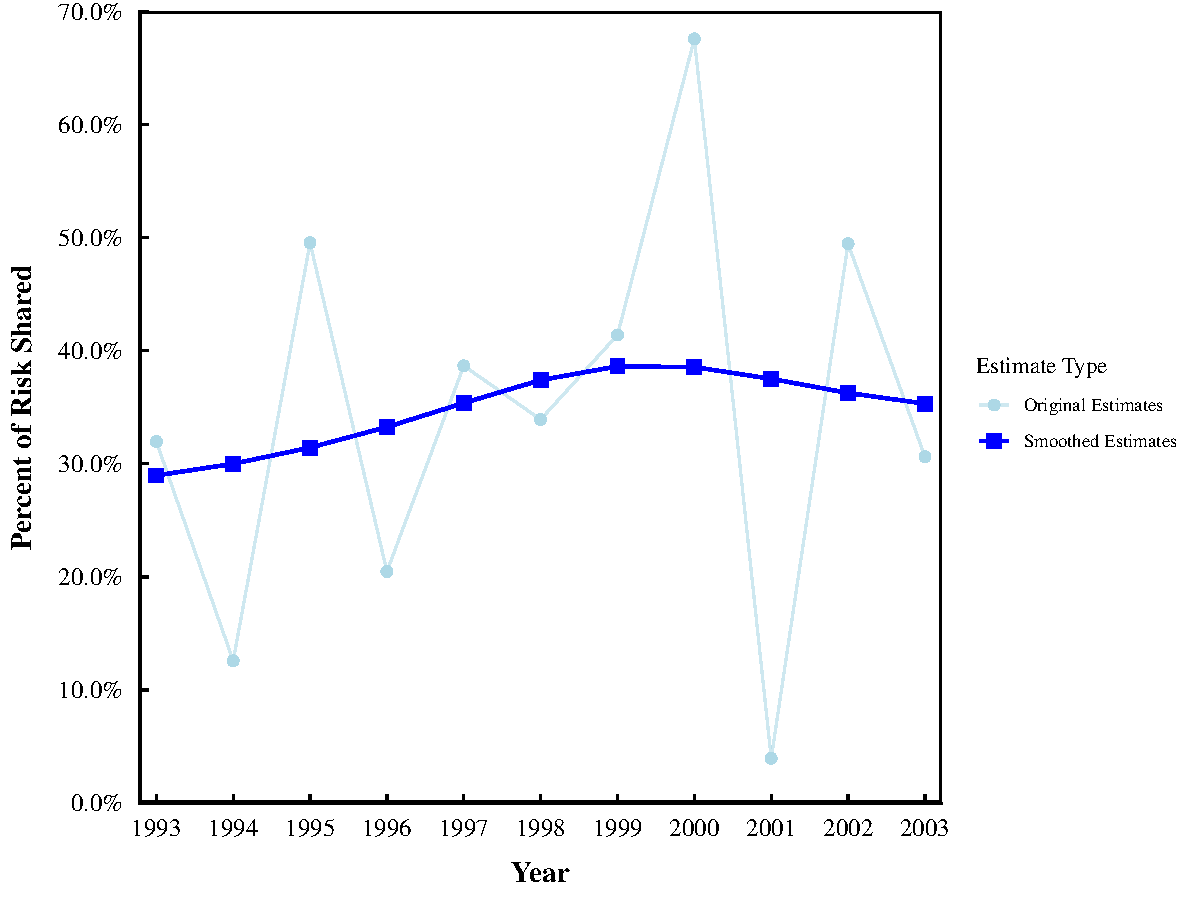
\includegraphics[width=\textwidth]{../output/rs_cs_rep_c.pdf}
        \caption{Replicated version}
    \end{subfigure}
    \hfill
    % Second subfigure
    \begin{subfigure}[b]{0.48\textwidth}
        \centering
        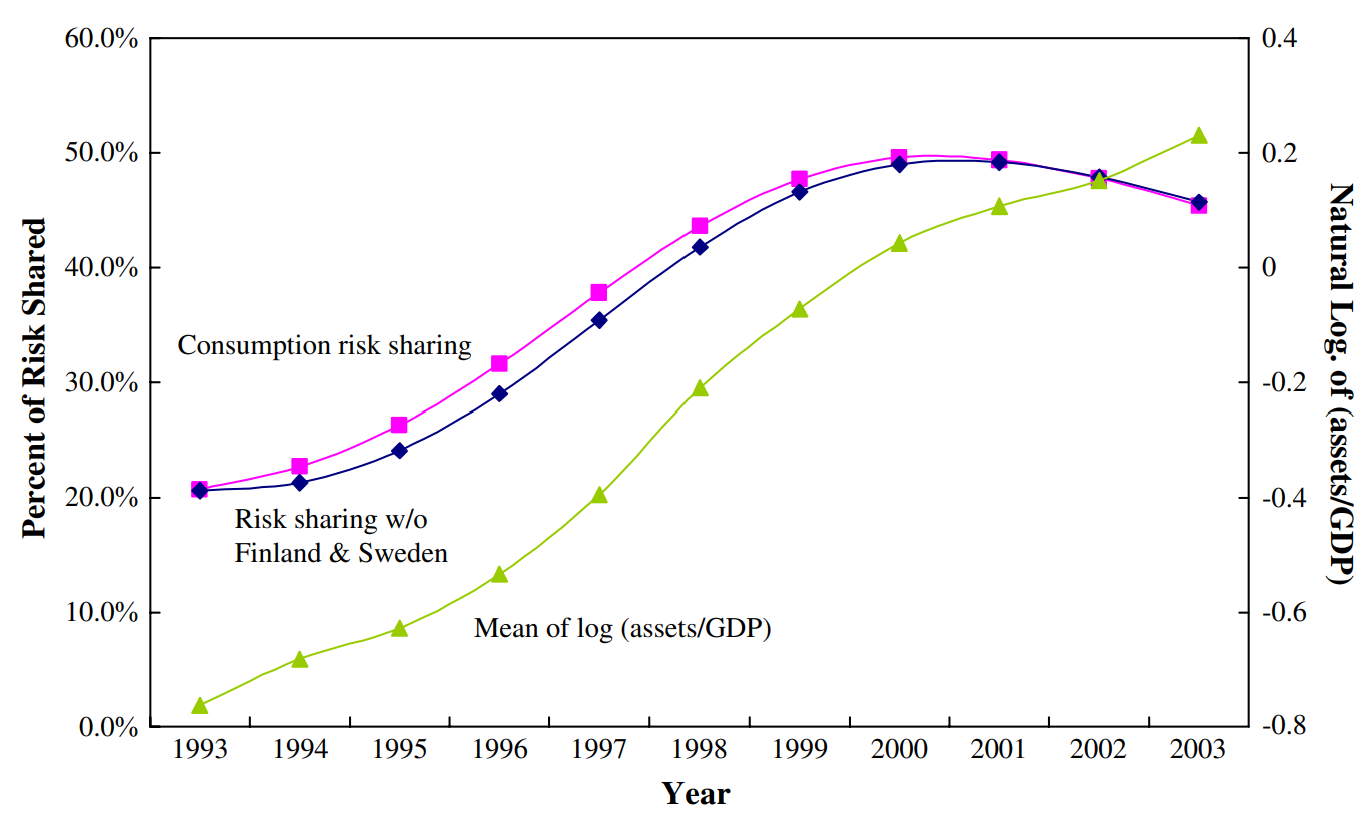
\includegraphics[width=\textwidth]{../output/main_fig_2.png}
        \caption{Original Paper}
    \end{subfigure}
    \hfill    
    \caption{Consumption Risk Sharing and foreign asset holdings}
\end{figure}

\newpage
% ============================================================
\section{Replication issues in Cross Section Risk Sharing}
% ============================================================
Throughout the process of our project, we were confronted with replicational difficulties
regarding the cross-sectional regressions displayed on the left of Figure \textbf{XXX}. While the choice of smoothing
parameters may influence the level and trend of the smoothed rik-sharing movement over time (see above), we also conclude the
analysis itself being highly sensitive to data chosen. This section is devoted to this sensitivity.\\
The authors of the reference paper describe how they gather GDP, GNI and consumption data in only 8 lines in the appendix \parencite[p.604]{main}.
Relying on OECD data, they manually compute real aggregate variables using 1995 (consumer) prices. As the cross-section regression compares 
variables not only across time but also countries, they calculate PPP-adjusted values using Purchasing Power Parities (i.e. exchange rates
accounting for differences in purchasing power across countries) provided by the OECD. Finally, they use population data to arrive at per capita values.\\
To show the sensitivity of the cross-sectional risk-sharing results, we replicated Figure 2 of \textcite{main} with three approaches, relying on OECD data for each of them.
First, we download GDP, GNI and consumption data from the OECD in current prices of the national currency. Using the country-specific CPIs, we convert to 2015 constant prices - the base 
year chosen by the OECD for most variables. We then use 2015 PPPs to arrive at PPP-adjusted data - all identical to the reference paper, with the exception of
the base year having changed from 1995 to 2015. Approach 2 uses OECD data of all variables already PPP-adjusted using chained-linked volumes, rebased to 2020. Chained linked volumes
are a the standard modern way of estimating real aggregates and recommended by the OECD over choosing a constant base year. Finally, extracting data published by the OECD in 2005 using 2000 as a constant base year,
we can construct Approach 3 most closely related to \textcite{main}, but with data that does not extend much the time period of the reference paper.\\
Approach 1 and the original version of the paper are in Panels A and B of Figure \textbf{XXX, above}, while approaches 2 and 3 are Panels A and B of Figure \textbf{XXX, below}.\\

\begin{figure}[htbp]
    \centering
    % First subfigure
    \begin{subfigure}[b]{0.48\textwidth}
        \centering
        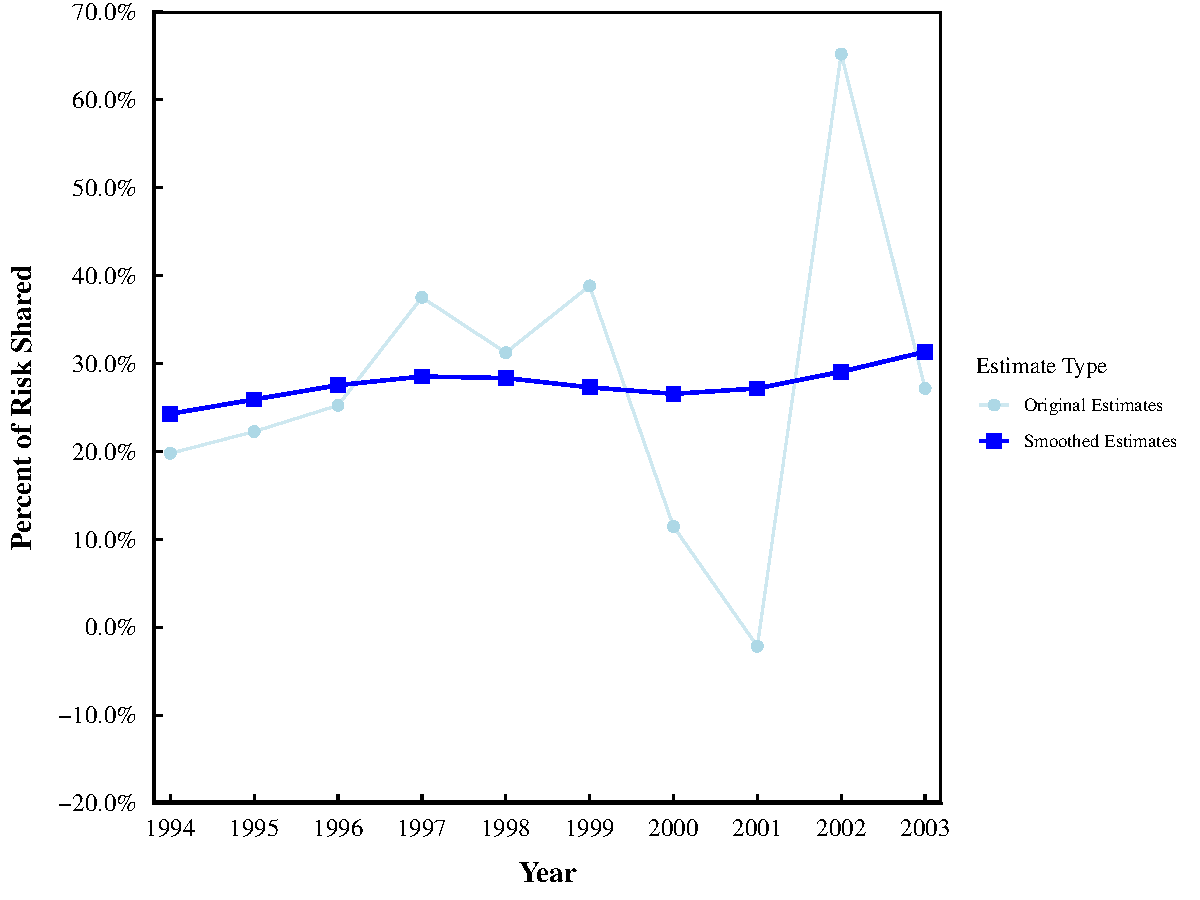
\includegraphics[width=\textwidth]{../output/rs_cs_sanity_c.pdf}
        \caption{2000 as base year (PDF-extracted data)}
    \end{subfigure}
    \hfill
    % Second subfigure
    \begin{subfigure}[b]{0.48\textwidth}
        \centering
        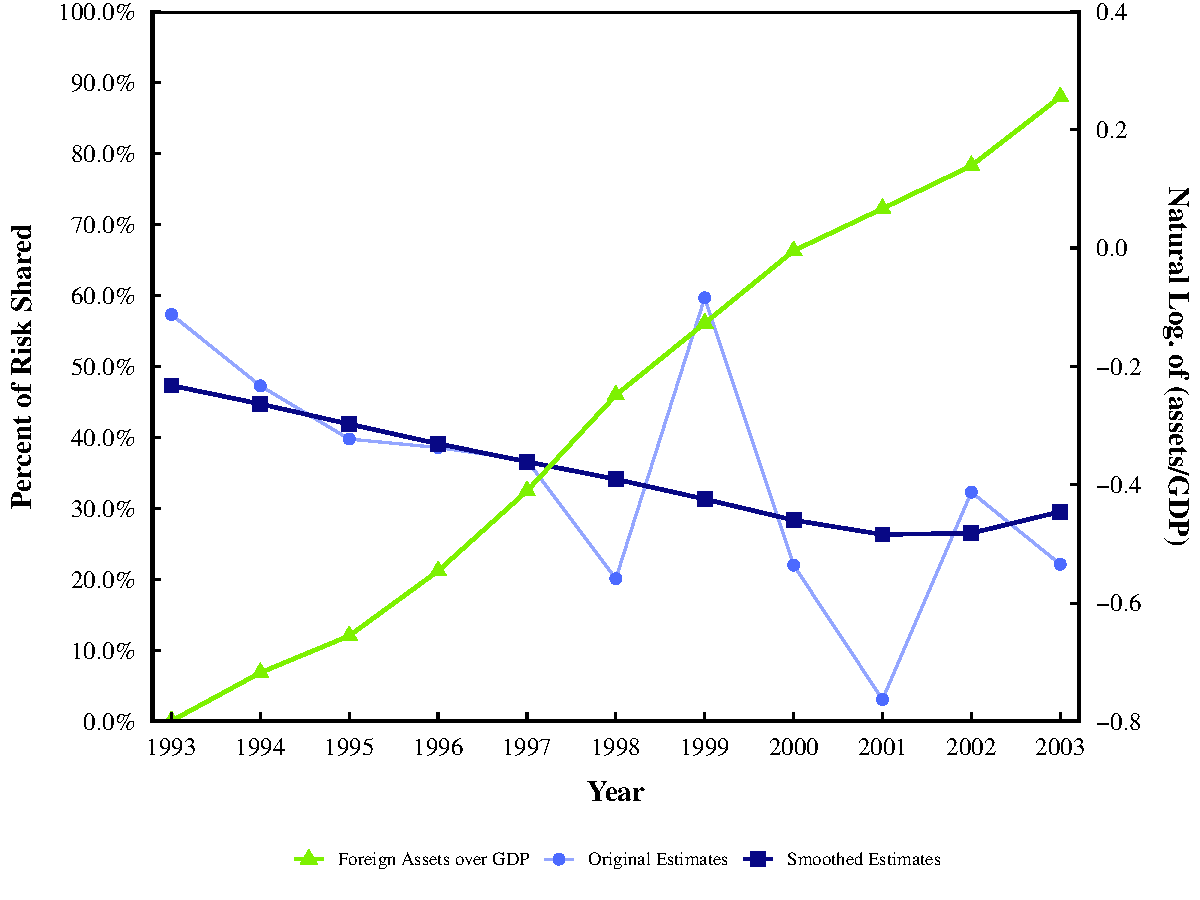
\includegraphics[width=\textwidth]{../output/rs_cs_rebased.pdf}
        \caption{Chained-linked volumes, 2020-rebased}
    \end{subfigure}
    \hfill    
    \caption{Consumption Risk Sharing (similar for GNI)}
\end{figure}

Most strikingly, using Approach 2, the trend of risk-sharing suddenly negative which would conclude the opposite of what the original paper claims.
We believe this sensitivity to the data chosen is partly reflected by the fact that using data rebased to 2020 for an estimation period from 1993 to 2003
has to account for changes in underlying economic fundamentals. As discussed during the presentation, this task is almost certainly bound to fail which is
why we conclude it to be worthwhile to get as close as possible to the base year chosen by the authors. Indeed, relying on 2000-constant prices gets us almost
perfectly close for GNI cross-section risk-sharing. For consumption risk sharing (see plot), we also get closer.\\
Hence, we decided to stick 2015 data, as we can replicate the original trend and are able to extend our analysis. We note this

\newpage
% ============================================================
\section{Investigating Eurozone Risk Sharing}
% ============================================================

The previously described data issues on EWN data notwithstanding, it might still be worthwhile to analyze how risk-sharing developed in the Euro Area. We devote this analysis to our final section.\\
\indent For a fist preliminary indication, consider Figure \textbf{XXX}. Used already multiple times, it displays the development of consumption risk sharing, 
using either Euro Area countries (Panels A) or non-Euro Area countries only (Panels B). Importantly, we depart from the baseline methodology by choosing the same aggregate for both subgroups.
As discussed in the presentation, using the same aggregate allows us to compare the shock insulation of EA countries with a non EA countries using the same baseline shock\footnote{Note that results do not differ much when using 
the within-group aggregate, see Appendix}.\\

Figure \textbf{XXX} shows the results. While it becomes apparent that between the introduction of the Euro in 1999 and the eve of the GFC in 2007, the increase in the Euro Area consumption risk sharing is more pronounced in the Euro Area sample, the difference
is comparatively low (30\% vs. 25\% increase). Furthermore, as explained in the first section, we argued that we regard the exact levels of risk sharing to be specification-sensitive. Hence, we may conclude that 
that consumption risk sharing has not markedly increased more in the Euro Area than in other countries.
\begin{figure}[htbp]
    \centering
    % Panel A
    \begin{subfigure}[b]{0.48\textwidth}
        \centering
        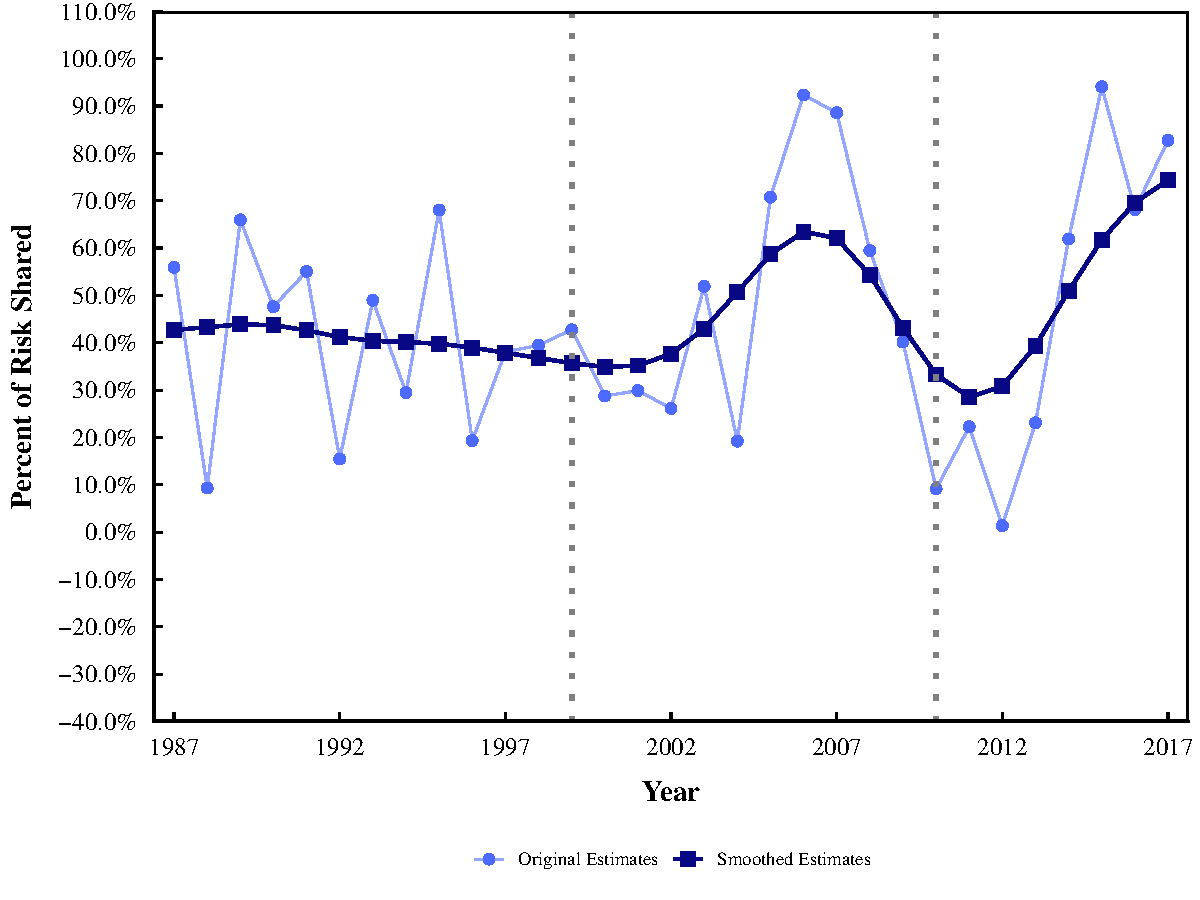
\includegraphics[width=\textwidth]{../output/rs_cs_ext_4_c.pdf}
        \caption{Eurozone only}
    \end{subfigure}
    \hfill
    % Panel B
    \begin{subfigure}[b]{0.48\textwidth}
        \centering
        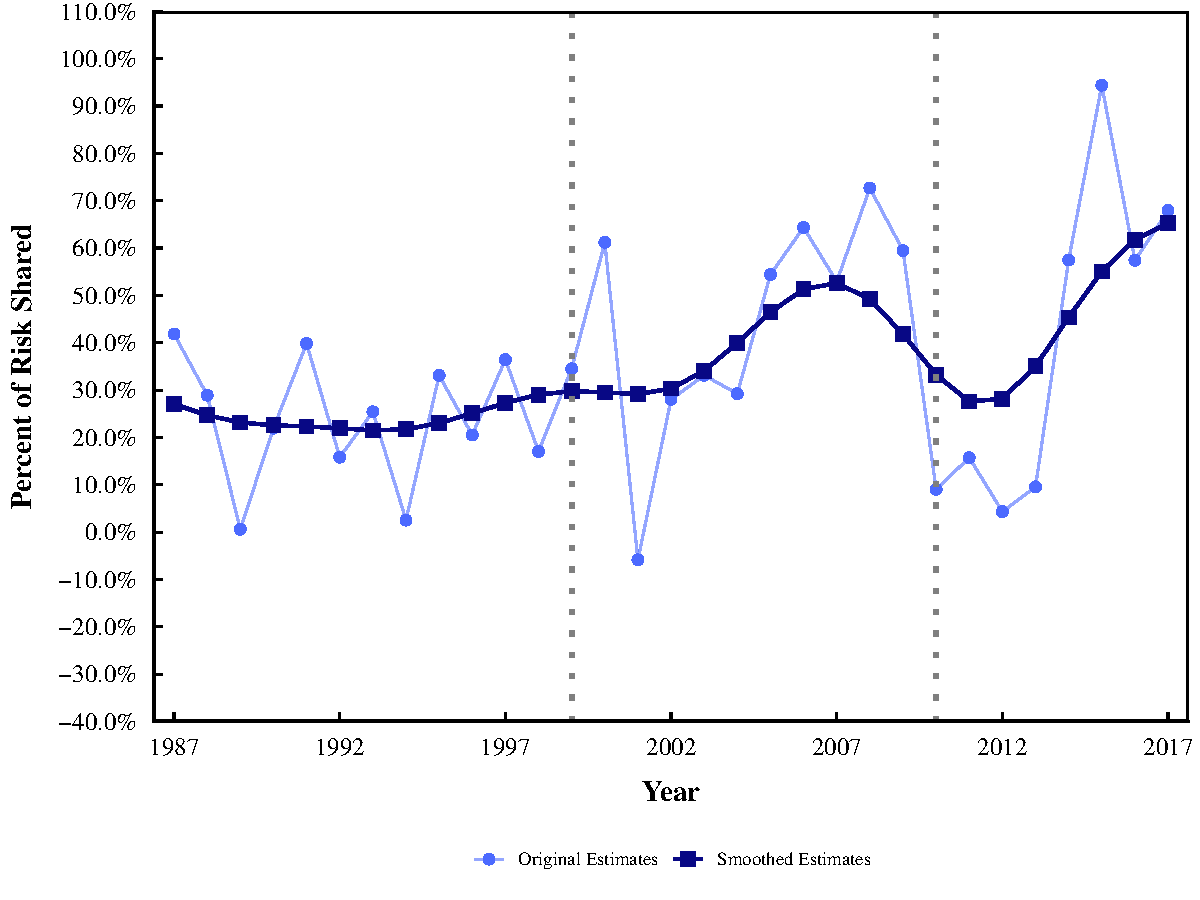
\includegraphics[width=\textwidth]{../output/rs_cs_ext_4b_c.pdf}
        \caption{Non-Eurozone}
    \end{subfigure}    
    \caption{Consumption Risk Sharing cross-sectional estimates (same aggregate)}
\end{figure}

\noindent To understand why we turn to a new set of methods, recall again our Euro Area hypothesis, inspired by the reference paper \textcite{main}.
With the introduction of the Euro in 1999, currency and transaction risks in the purchase of Euro Area assets disappeared such that the Euro Area Home Bias
should fall and fall more than in other countries. Relying on \textbf{Working Paper}, we were able to confirm this only for the Debt Home Bias.
We may therefore expect that the total Home Bias did not fall enough for Europe to experience a large increase in risk sharing. While the graphical analysis above
provided some evidence on that, we turn to yet another method to test this unexpected result again.\\
\indent \textcite{asy1996} develop a convincing method to isolate different channels of risk sharing, helping us to test our hypothesis without relying on the shaky EWN data. The method builds on the chain 
between GDP, GNI, Gross National Disposable Income (GDI) and Consumption using:
\begin{equation}
    \mathrm{GDP}_{it} = \frac{\mathrm{GDP}_{it}}{\mathrm{GNI}_{it}}\frac{\mathrm{GNI}_{it}}{\mathrm{GDI}_{it}}\frac{\mathrm{GDI}_{it}}{\mathrm{C}_{it}}\mathrm{C}_{it}
\end{equation}
Taking logs and differencing, one arrives at:
\begin{align}
    \Delta \log \mathrm{GDP}_{it} = & (\Delta \log \mathrm{GDP}_{it} - \Delta \log \mathrm{GNI}_{it}) + (\Delta \log \mathrm{GNI}_{it} - \Delta \log \mathrm{GDI}_{it}) + \\
    & (\Delta \log \mathrm{GDI}_{it} - \Delta \log \mathrm{C}_{it}) + \Delta \log \mathrm{C}_{it} \notag
\end{align}
Proceed by evaluating \textbf{(XX)} at the cross-sectional mean and subtracting it from \textbf{(XX)}. Multiplying with $(\Delta \log \mathrm{GDP}_{it} - \Delta \log \overline{\mathrm{GDP}_{t}})$ 
and evaluating in expectation gives:
\begin{align}
    \mathrm{Var}(\Delta \log \mathrm{GDP}_{it}) = & \mathrm{Cov}(\Delta \log \mathrm{GDP}_{it} - \Delta \log \mathrm{GNI}_{it}, \Delta \log \mathrm{GDP}_{it}) + \\
    & \mathrm{Cov}(\Delta \log \mathrm{GNI}_{it} - \Delta \log \mathrm{GDI}_{it}, \Delta \log \mathrm{GDP}_{it}) + \notag \\
    & \mathrm{Cov}(\Delta \log \mathrm{GDI}_{it} - \Delta \log \mathrm{C}_{it}, \Delta \log \mathrm{GDP}_{it}) + \mathrm{Cov}(\Delta \log \mathrm{C}_{it}, \Delta \log \mathrm{GDP}_{it}) \notag
\end{align}
Finally, we may divide by the left-hand side to arrive at an equation including four simple OLS-coefficients that, by construction, sum to one:
\begin{equation}
    \beta_C + \beta_F + \beta_C + \beta_U = 1.
\end{equation}
Consider just the first coefficient. It is identified by the OLS-regression $\Delta \log \mathrm{GDP}_{it} - \Delta \log \mathrm{GNI}_{it}= \alpha_C + \beta_C \Delta \log \mathrm{GDP}_{it} + \epsilon_{it}$. Its coefficient therefore measures the
degree to which idiosyncratic output growth can explain the growth differential between GDP and GNI. As the difference between GDP and GNI relates to net factor income from abroad, \textcite{asy1996} interpret $\beta_C$ as the 
amount of risk-sharing obtained via cross-ownership of assets, i.e. capital markets. Similarly, we may interpret $\beta_F$, $\beta_C$ and $\beta_U$ as the amount
of risk sharing obtained via federal transfers, credit markets (borrowing/ lending) and an unsmoothed residual, respectively.\\

We may now make use of this methodology to relate it back to our hypothesis. If indeed the introduction of a common currency lead to a reduction in the 
Eurozone Home Bias, the share of consumption risk sharing achieved via capital markets should increase over time.\\
To test this hypothesis, we first gather the same data as the well-documented working paper \textcite{working_paper_26}. We are able to replicate both Table 7 and Figure 4,
which runs Panel and Cross-Section Regressions for an EU27 sample and use this to reassure us of the correct methodological implementation. Then, we restrict ourselves to the Euro Area and construct year-by-year
estimates of different risk sharing channels in the Euro Area, plotted in Figure \textbf{XXX}, constructed equivalently to \textcite[p.23]{working_paper_26}.
\begin{figure}[htbp]
    \centering
    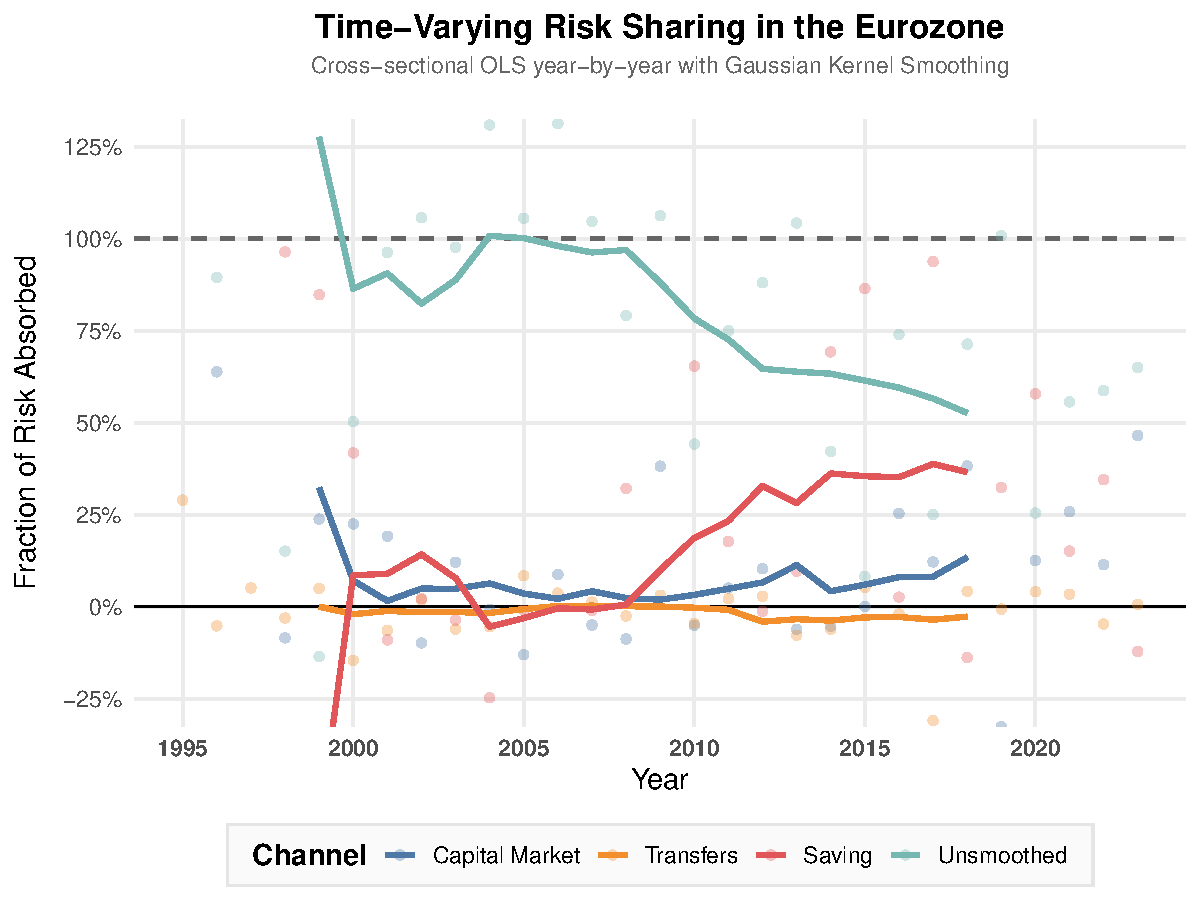
\includegraphics[width = 0.5\textwidth]{../output/channels_cross_section.pdf}
    \caption{Year-by-year cross-sectional estimates (Smoothed with 10-year centred moving averages)}
\end{figure}

\noindent Graphically, it becomes evident that the capital markets channel behaves almost flat. It slowly decreases until the GFC and slowly increases shortly after.
While it does turn significant when running Panel Regressions for 2010-2023 (see Appendix), it is not for the period 1995-2007. Hence, the mere abolishment of exchange-rate risk
most likely did not reduce the Home Bias enough to increase consumption risk sharing in the Euro Area.\\
We may relate this finding back to the literature and our reference paper. As described in \textcite[p.214]{sy1998}, "If capital controls and cost of transacting in many currencies
have been the main cause of little cross-country
ownership, their removal may induce a swift process of capital market integration." Evidently, our analysis shows that capital market integration, if significant, has neither been sizeable nor swift.
Second, as hypothesized already in our reference paper, "hedging of currency risk is not the main reason for home bias" \parencite[p.591]{main}. Again, we can confirm that neither of our extensions seems to disprove this statement.\\

Our conclusion stresses the main tradeoff from the Optimum Currency Area literature, briefly covered in the lecture. Forming a currency union comes at the cost of having to 
agree on a common monetary policy, such that member states cannot react with interest rate or exchange rate adjustment following idiosyncratic shocks. Our report confirms doubts in the cited literature
that the reduction of currency risk provides enough incentives to acquire cross-border assets (i.e. reduce the Home Bias). The Euro Area should therefore make it a priority to increase risk sharing through
other measures to get closer to US interstate levels (a successful monetary union) where only around 20\% of output shocks are unsmoothed and capital markets smooth more than 50\% of consumption.  
\newpage

\printbibliography

\newpage

\begin{figure}[htbp]
    \centering
    \begin{minipage}[b]{0.48\textwidth}
      \centering
      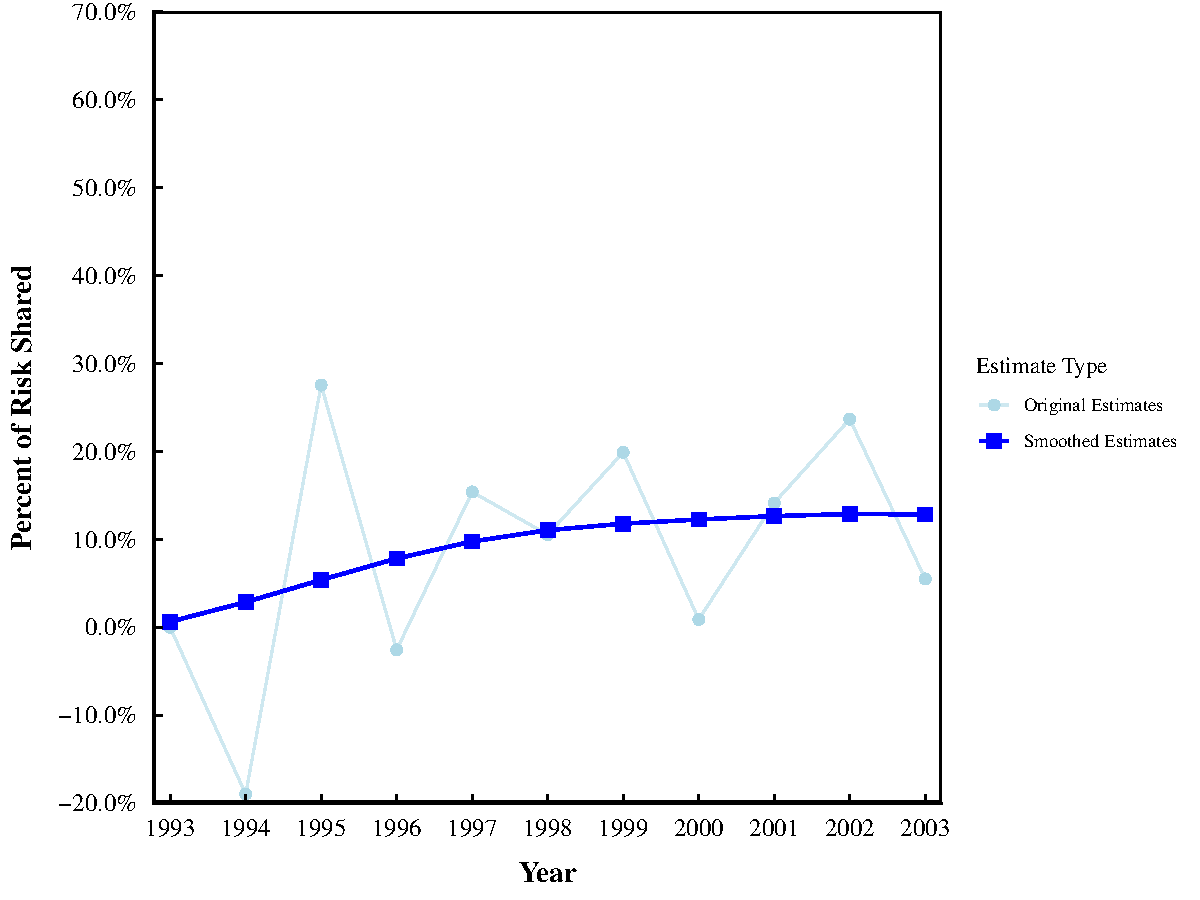
\includegraphics[width=\textwidth]{../output/rs_cs_rep_i.pdf}
    \end{minipage}\hfill
    \begin{minipage}[b]{0.48\textwidth}
      \centering
      \raisebox{0.7cm}{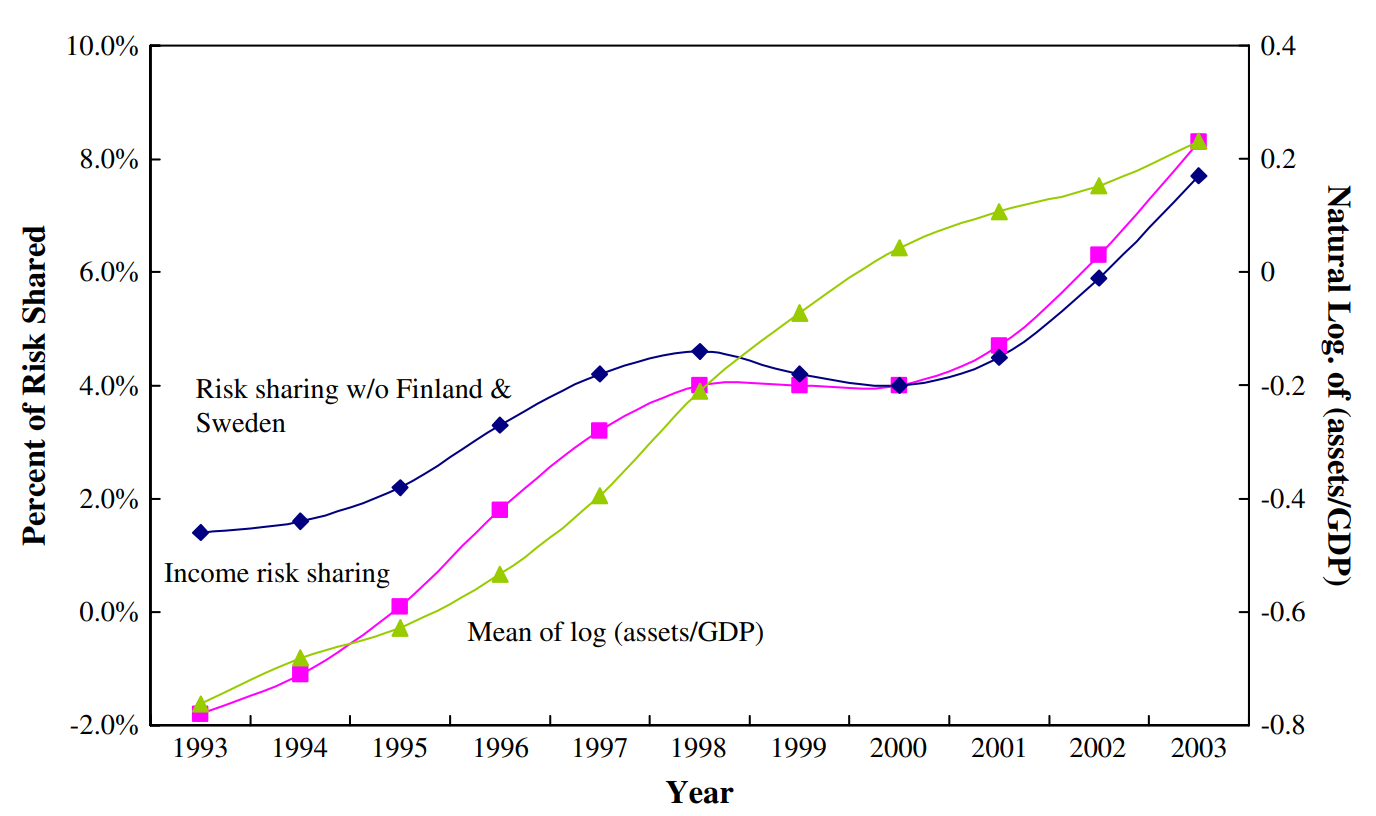
\includegraphics[width=\textwidth]{../output/main_fig_1.png}}
    \end{minipage}
    \caption{Income Risk Sharing and foreign asset holdings}
\end{figure}

\begin{figure}[htbp]
    \centering
    % Panel A
    \begin{subfigure}[b]{0.48\textwidth}
        \centering
        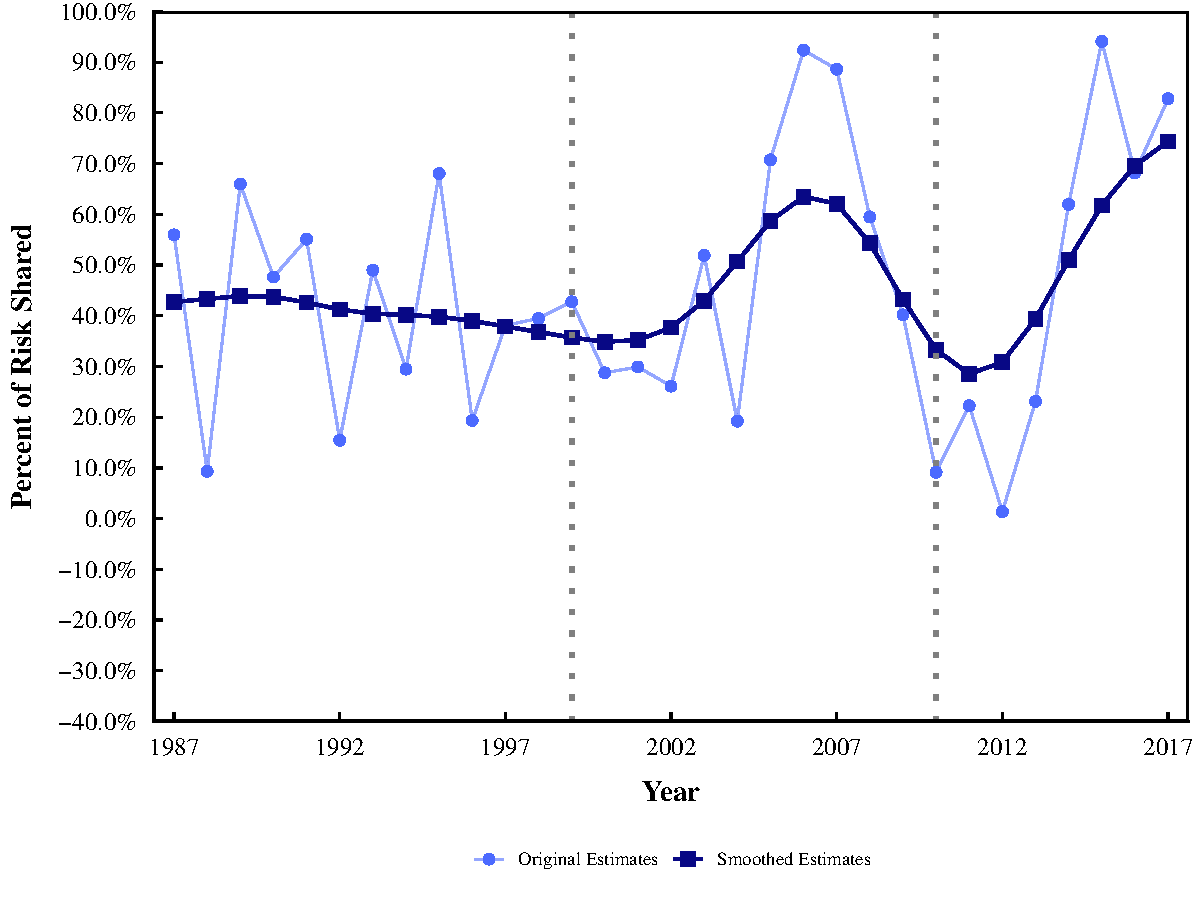
\includegraphics[width=\textwidth]{../output/rs_cs_ext_3_c.pdf}
        \caption{Eurozone only - Consumption}
    \end{subfigure}
    \hfill
    % Panel B
    \begin{subfigure}[b]{0.48\textwidth}
        \centering
        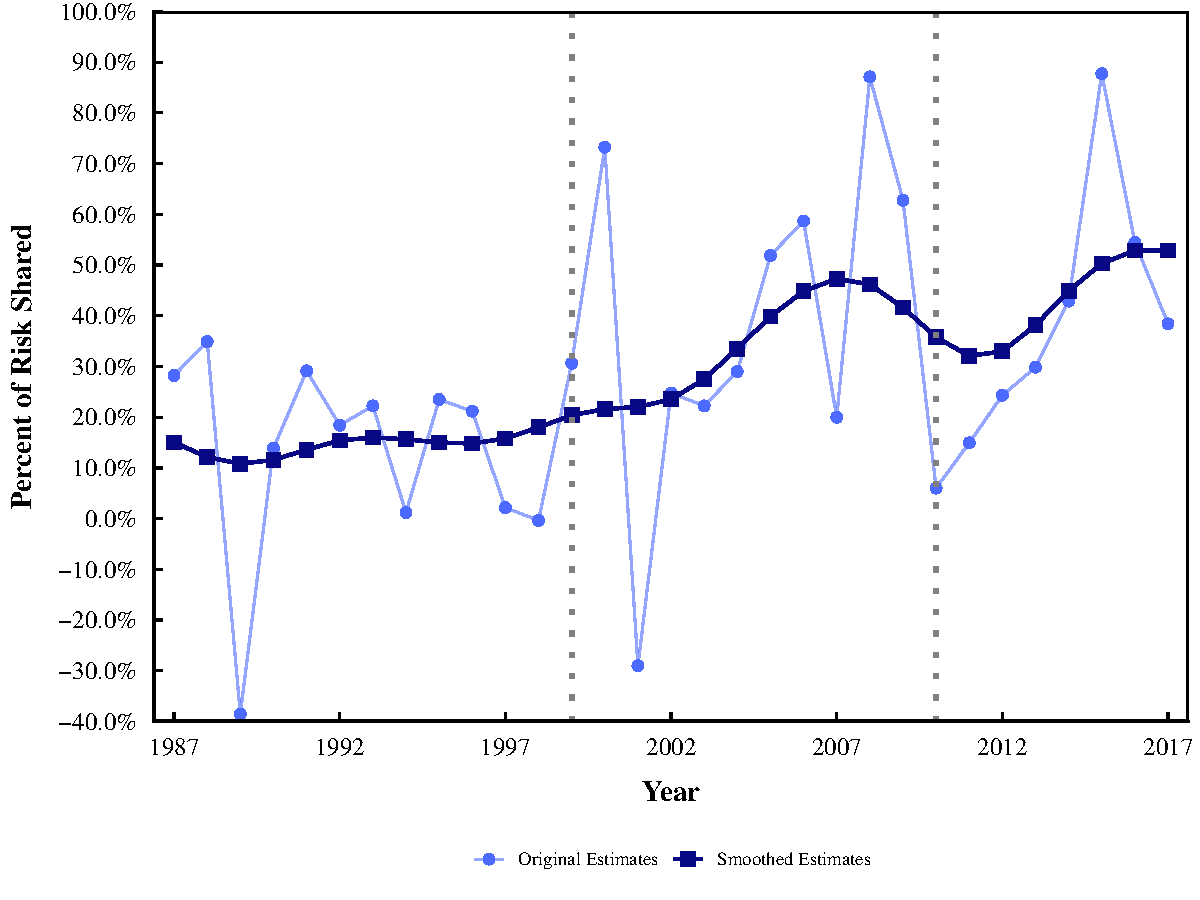
\includegraphics[width=\textwidth]{../output/rs_cs_ext_3b_c.pdf}
        \caption{Non-Eurozone - Consumption}
    \end{subfigure}
    \caption{Risk Sharing cross-sectional estimates for selected subgroups (Within-group aggregates)}
\end{figure}

\begin{figure}[htbp]
    \centering
    % First subfigure
    \begin{subfigure}[b]{0.48\textwidth}
        \centering
        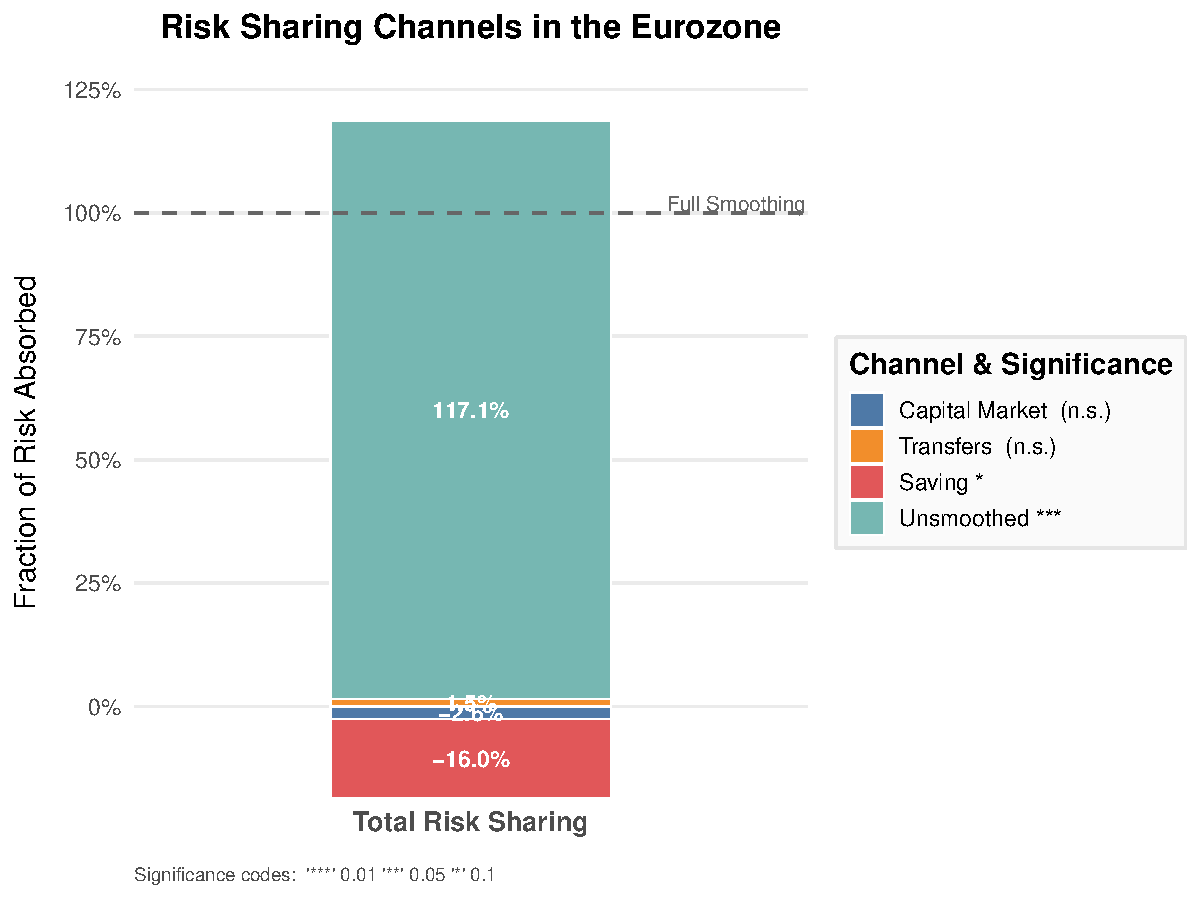
\includegraphics[width=\textwidth]{../output/ea_95_07.pdf}
        \caption{1995 -- 2007}
    \end{subfigure}
    \hfill
    % Second subfigure
    \begin{subfigure}[b]{0.48\textwidth}
        \centering
        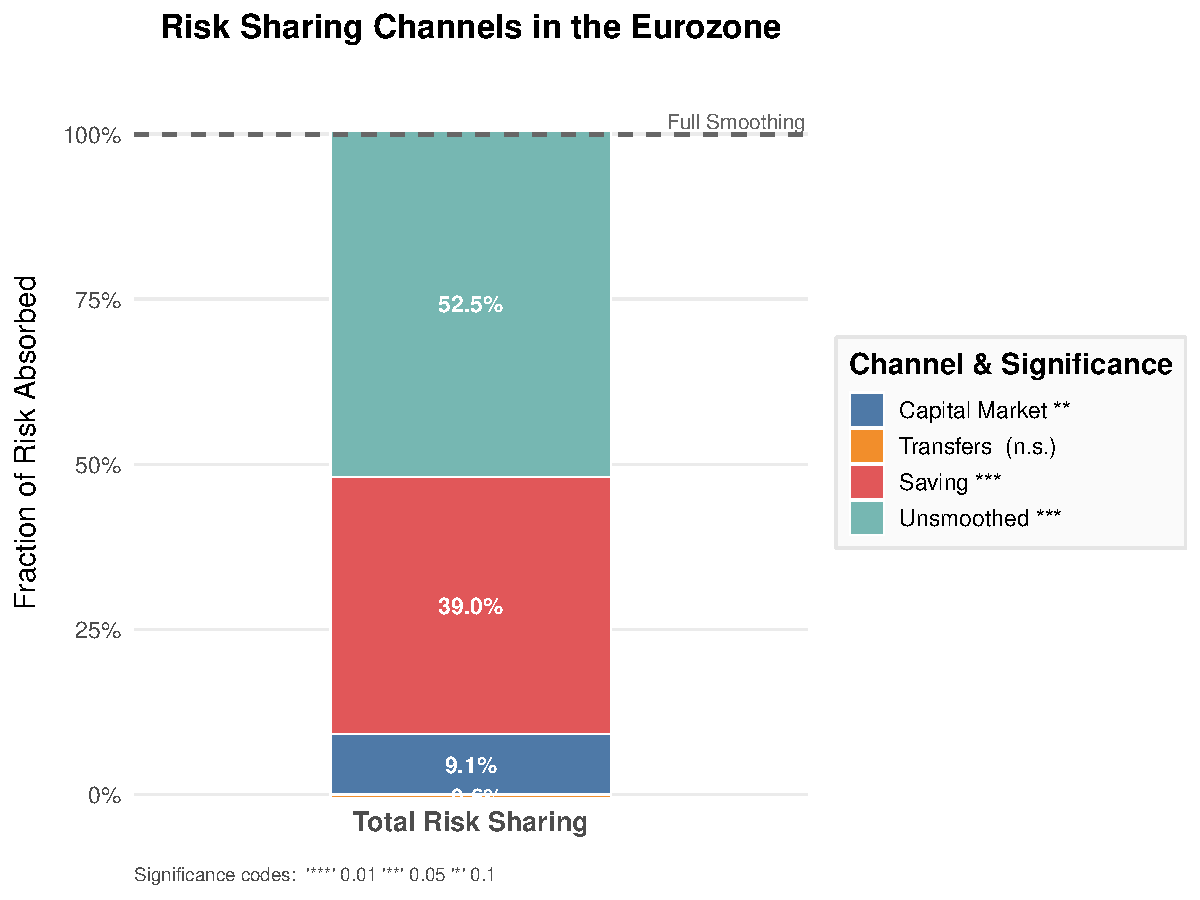
\includegraphics[width=\textwidth]{../output/ea_10_23.pdf}
        \caption{2010 -- 2023}
    \end{subfigure}
    \hfill    
    \caption{Risk Sharing Channels (Panel estimation) across different time periods}
\end{figure}

\end{document}